\documentclass[12pt]{article}
\usepackage[utf8]{inputenc}
\usepackage{graphicx}
\usepackage{fixltx2e}
\graphicspath{{images/}}
\usepackage{float}
\usepackage[magyar]{babel}
\title{Rendszer- és irányításelmélet esti 2017-18 tavasz házi feladat}
\author{Benkő Gábor}
\date{\today}
\begin{document}
\maketitle
\newpage
\section{Empirikus szabályozótervezés}
\subsection{Szabályozó tervezés Ziegler-Nichols kísérleti identifikáción alapuló szabályozás módszerével}
\begin{figure}[h]
    \centering
	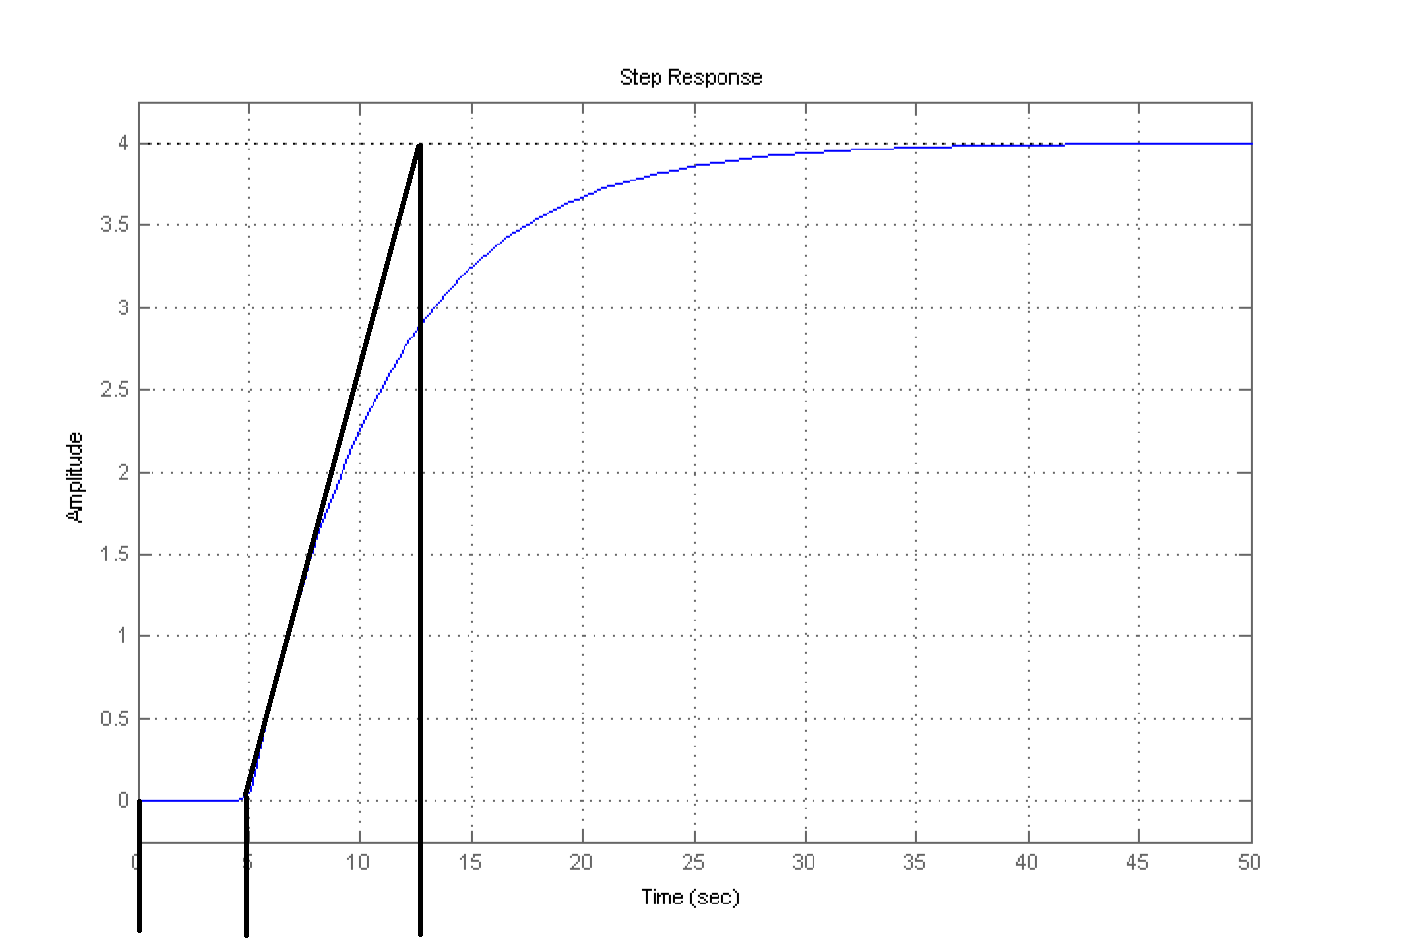
\includegraphics[scale=.4]{stepresponse}
	\caption{A szabályozandó rendszer ugrásválasza}
	\label{fig:stepresponse}
\end{figure}
Az ábrán látható megadott ugrásválasz alapján kerül tervezésre a PID szabályozó. Az ugrásválasz alapján az identifikáció alapján az alábbi értékek kerültek kinyerésre:
\begin{center}
\begin{tabular}{|c c c|}
\hline Név & Jelölés & Érték \\
\hline \hline
Holtidő & T\textsubscript{u} & 4\textsubscript{s} \\
\hline
Felfutási idő & T\textsubscript{r} & 12\textsubscript{s} \\
\hline
A szakasz erősítése & K\textsubscript{p} & 4 \\
\hline
\end{tabular}
\end{center}
Az eredményekből kiszámolásra került a $\rho=\frac{T_u}{T_r}=\frac{4}{13}=0.3333$ értéke, illetve a $T_I=2*T_U=8$ és a $T_D=T_U=4$. Az $A_p$ értéke kiszámolása a $A_p*K_p*\rho\leq1.2$ egyenlet átrendezésével \[A_P\leq\frac{1.2}{K_P*\rho}\leq0.9000\]
A PID szabályozó átviteli függvénye \[W\textsubscript{PID}=0.9000*(1+\frac{1}{8s}+4s)\]
ahol a MATLAB alapján keletkezett átviteli függvény \[W\textsubscript{PID}=\frac{3.6s^2+0.9s+0.1125}{s}\].
A Simulink-ban létrehozott rendszer ugrásválasza:
\begin{figure}[H]
\centering
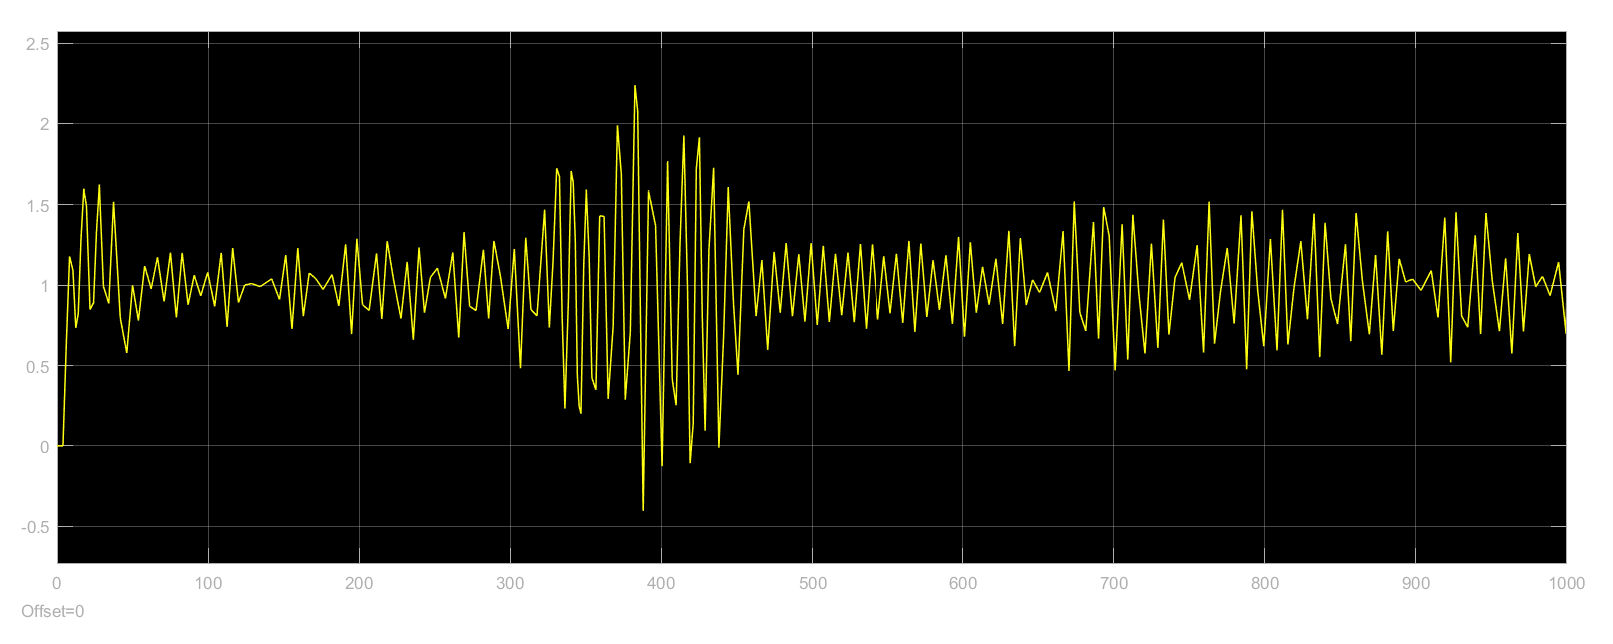
\includegraphics[scale=.50]{zgpidosc}
\caption{Az $A_P=0.9000$ rendszer ugrásválasza}
\end{figure}
Az ugrásválasz alapján látható a rendszer a stabilitás határán van. Ha rendszer stabilan szeretnénk tartani akkor $A_P<0.9000$ kell lennie. Így empirikus módszer segítségével csökkentjük az erősítési tényezőt, amíg megtaláljuk a közeli erősítési tényezőt.
A felezési módszertannal $A_P=0.1000$ esetén:
\begin{figure}[H]
\centering
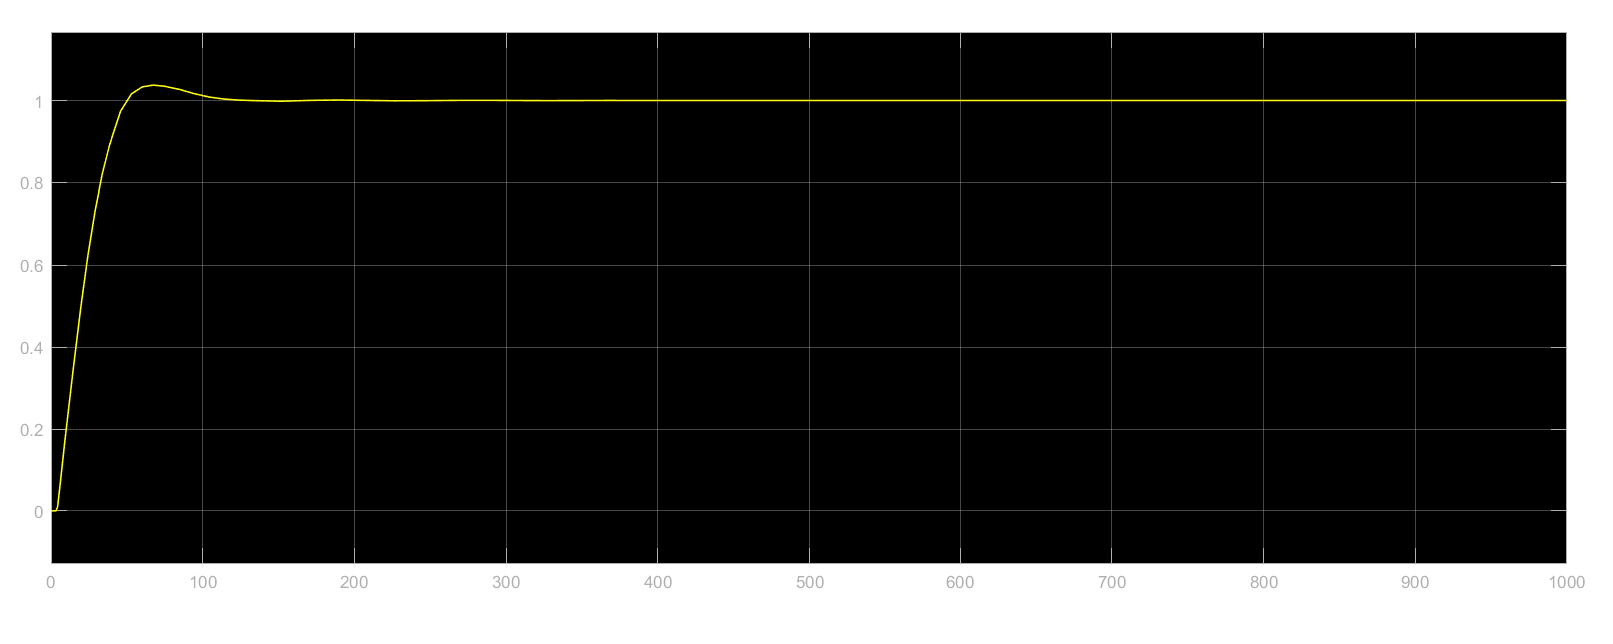
\includegraphics[scale=.50]{ap0100}
\caption{Az $A_P=0.1000$ rendszer ugrásválasza}
\end{figure}
a rendszerünk már stabil, illetve van egy kis túllövése, mely után beáll állandósult állapotba. A rendszer erősítését így tovább növelhetjük. A felezési módszer alapján, most az $A_P=0.4500$ erősítés esetén:
\begin{figure}[H]
\centering
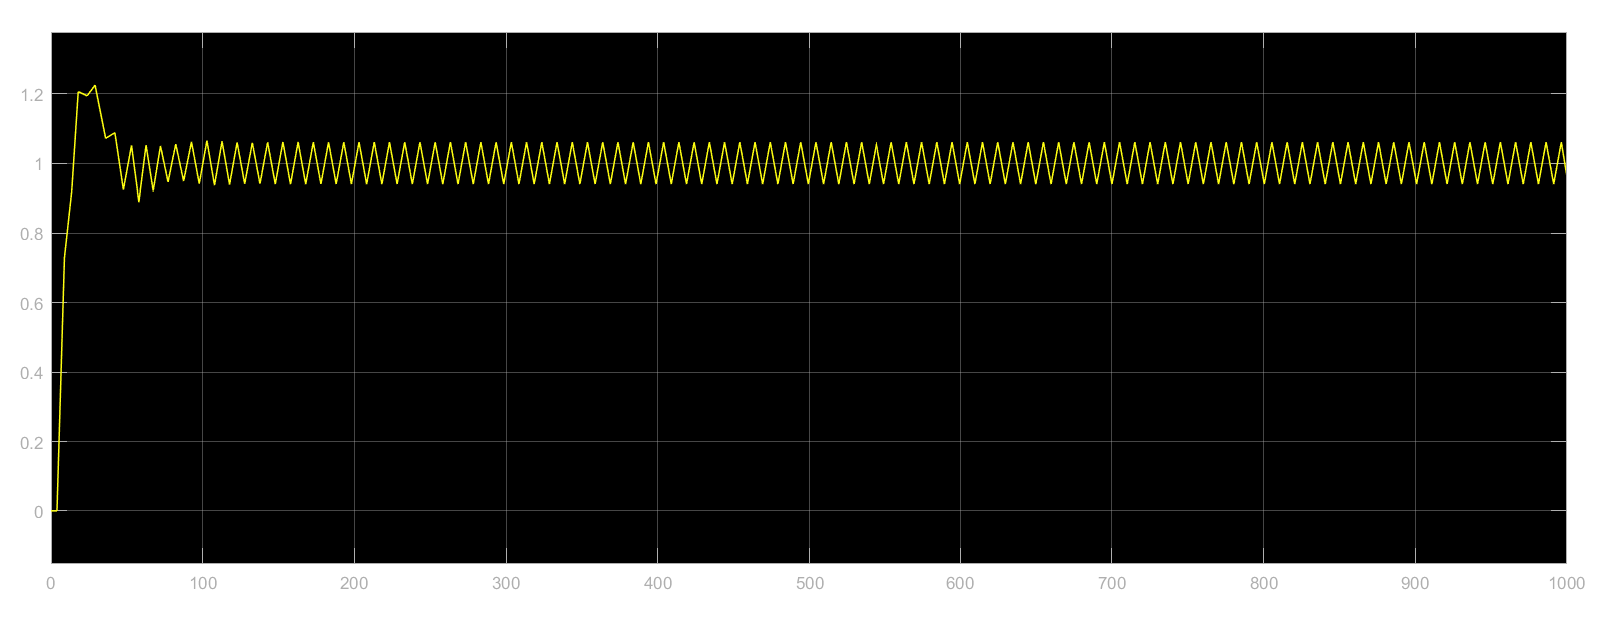
\includegraphics[scale=.50]{ap0450}
\caption{Az $A_P=0.4500$ rendszer ugrásválasza}
\end{figure}
A rendszer most a stabilitás határán van, így az erősítés tényezőt csökkentem $A_P=0.225$ értékre.
\begin{figure}[H]
\centering
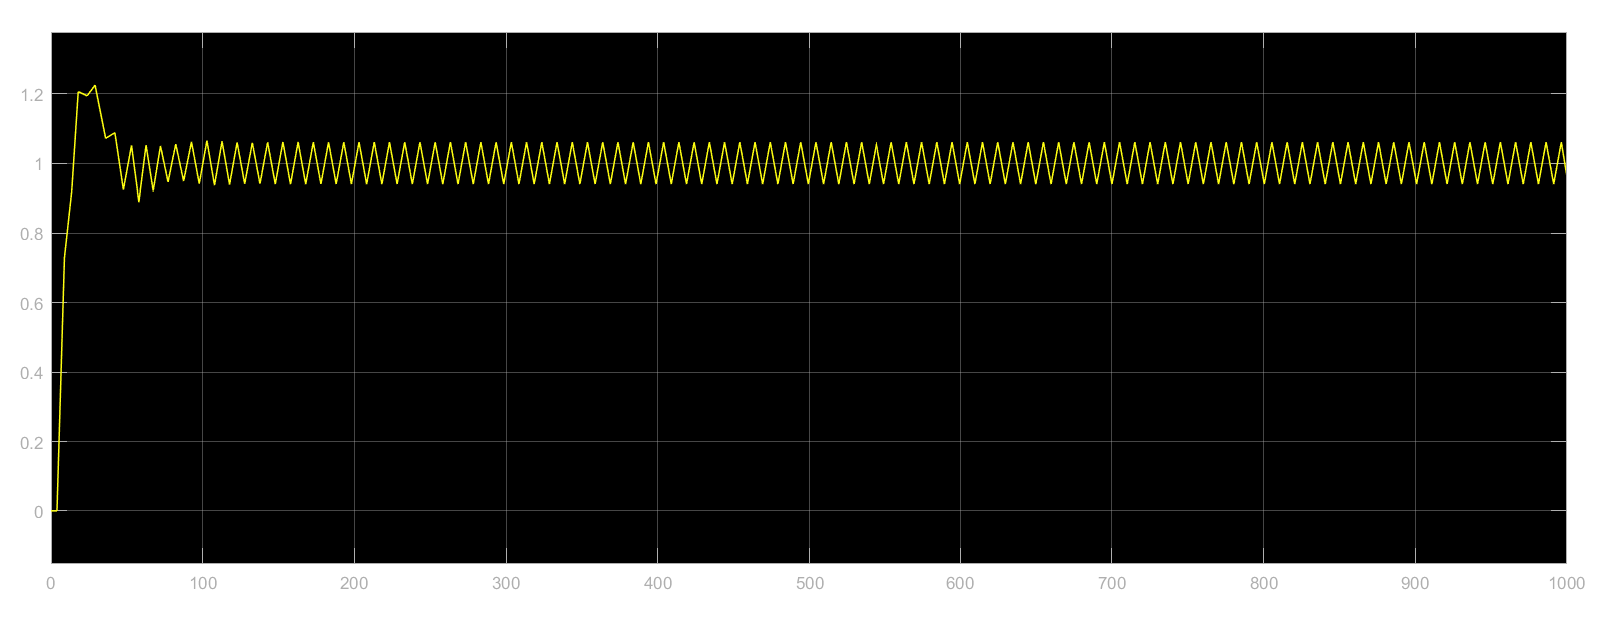
\includegraphics[scale=.50]{ap0450}
\caption{Az $A_P=0.2250$ rendszer ugrásválasza}
\end{figure}
A rendszer $A_P=0.2250$ estén stabil és van túllövése. Az $A_P$ értéke növelhető $A_P=0.337$.
\begin{figure}[H]
\centering
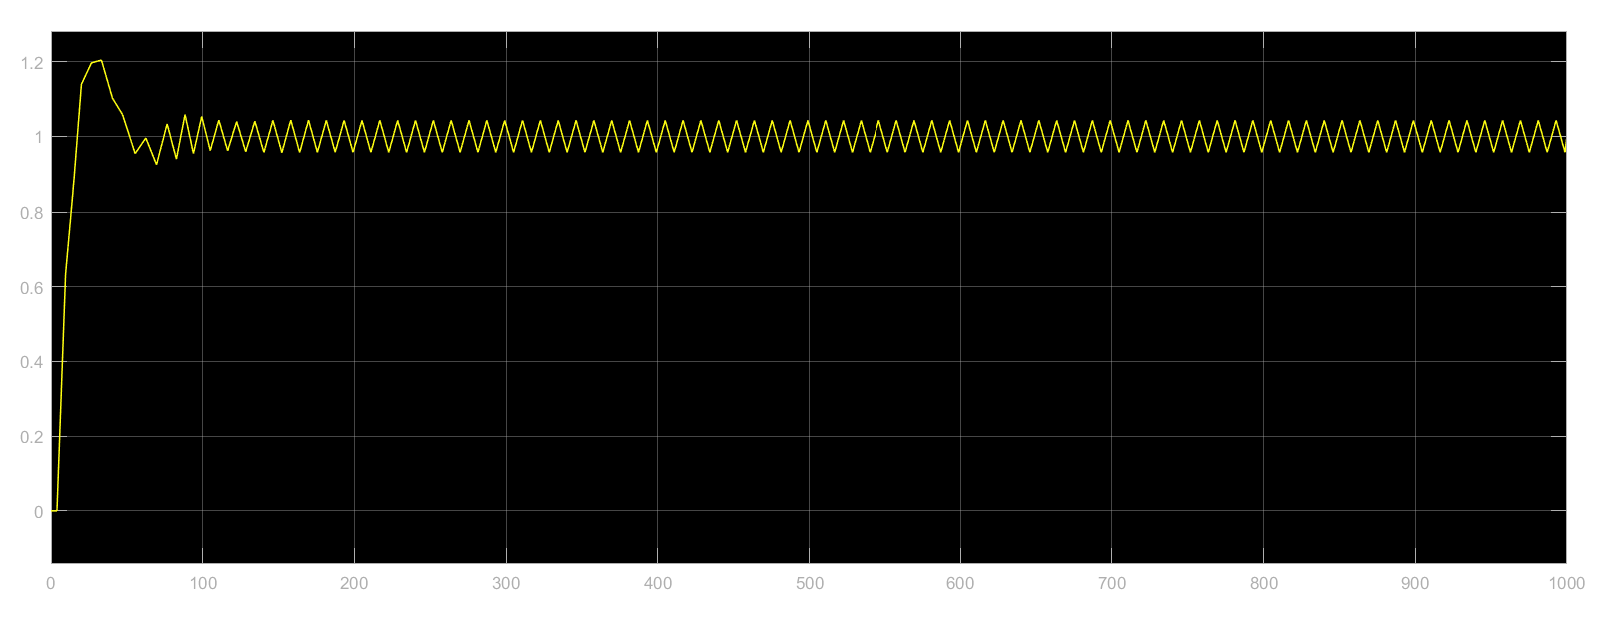
\includegraphics[scale=.50]{ap337}
\caption{Az $A_P=0.3370$ rendszer ugrásválasza}
\end{figure}
A rendszer a stabilitás határán van, így az $A_P=0.2810$ értékre csökkentve az ugrásválasz:
\begin{figure}[H]
\centering
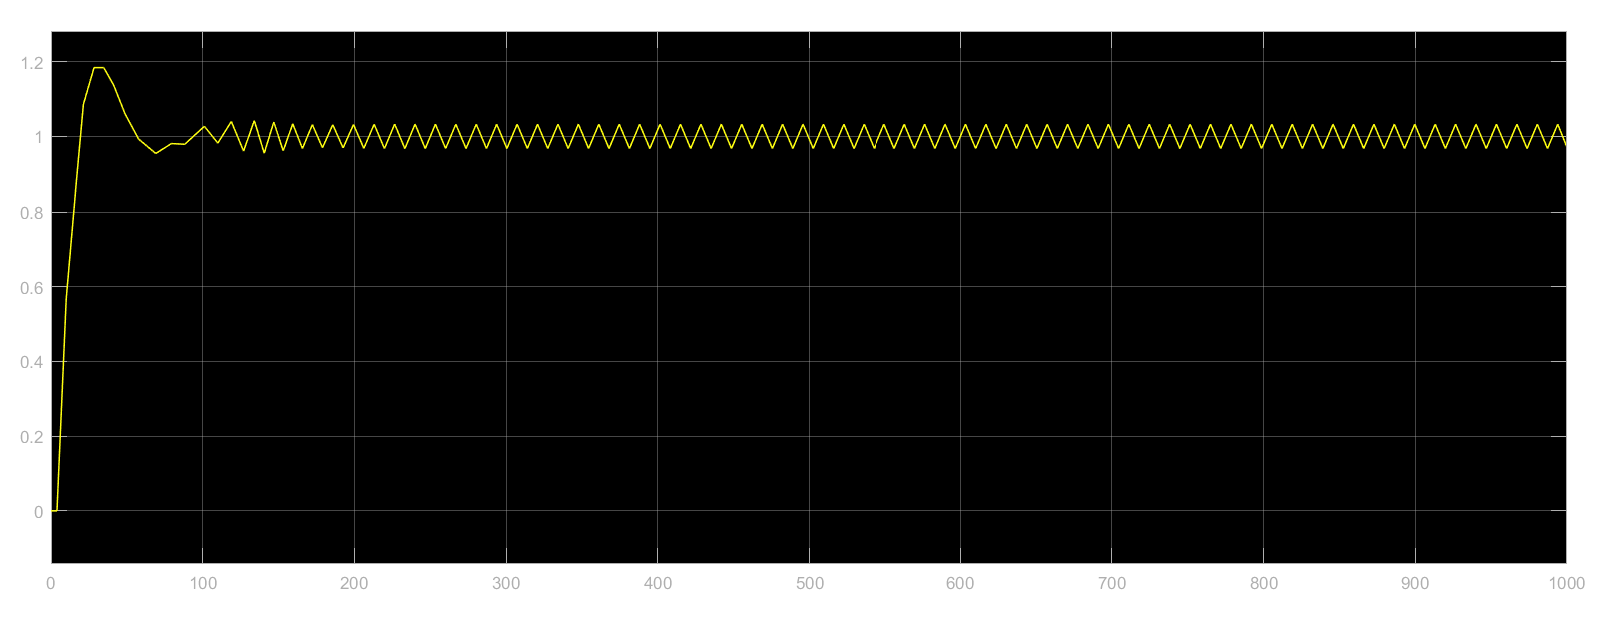
\includegraphics[scale=.50]{ap02810}
\caption{Az $A_P=0.2810$ rendszer ugrásválasza}
\end{figure}
A rendszer a stabilitás határán van továbbra is, így az $A_P$ értékét $A_P=0,2530$-ra csökkentem.
\begin{figure}[H]
\centering
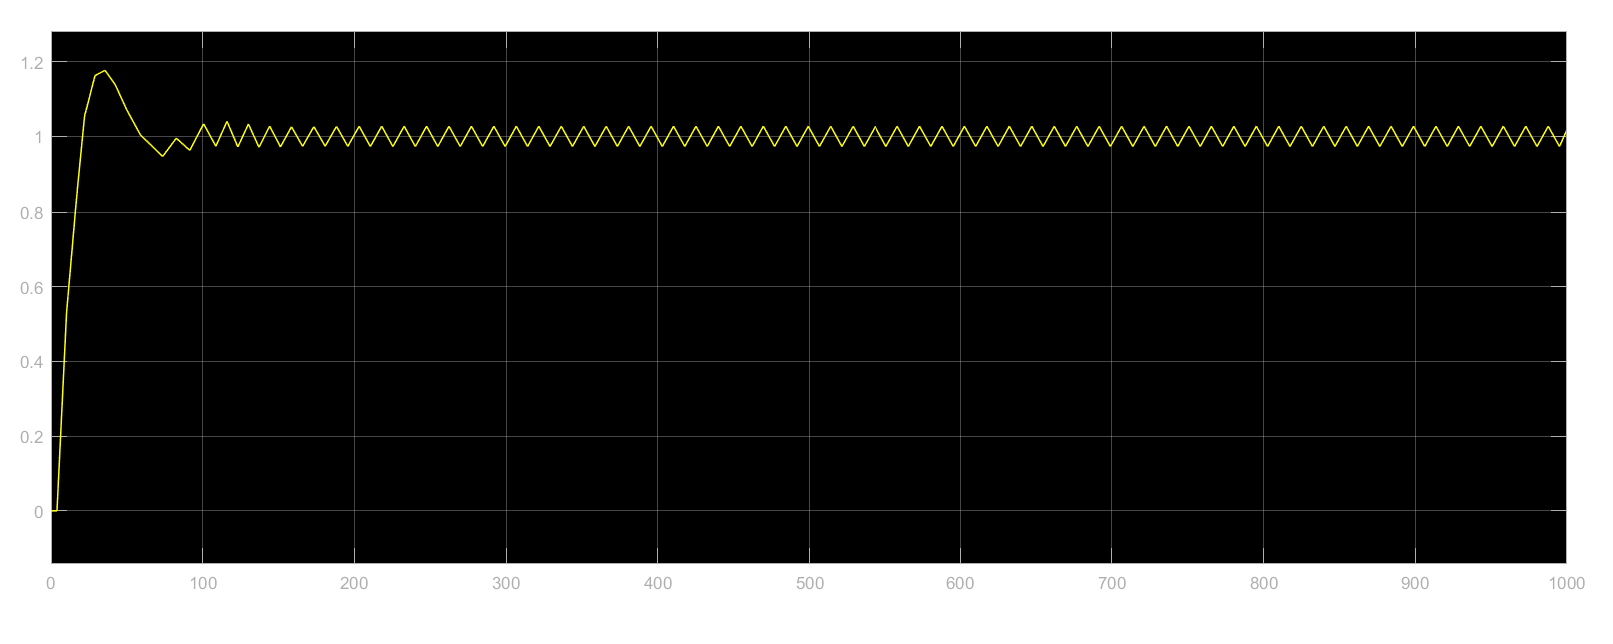
\includegraphics[scale=.50]{ap0253}
\caption{Az $A_P=0.2530$ rendszer ugrásválasza}
\end{figure}
A rendszer továbbra is stabilitás az határán, így az $A_P$ értékét $A_P=0.2390$-re csökkentem.
\begin{figure}[H]
\centering
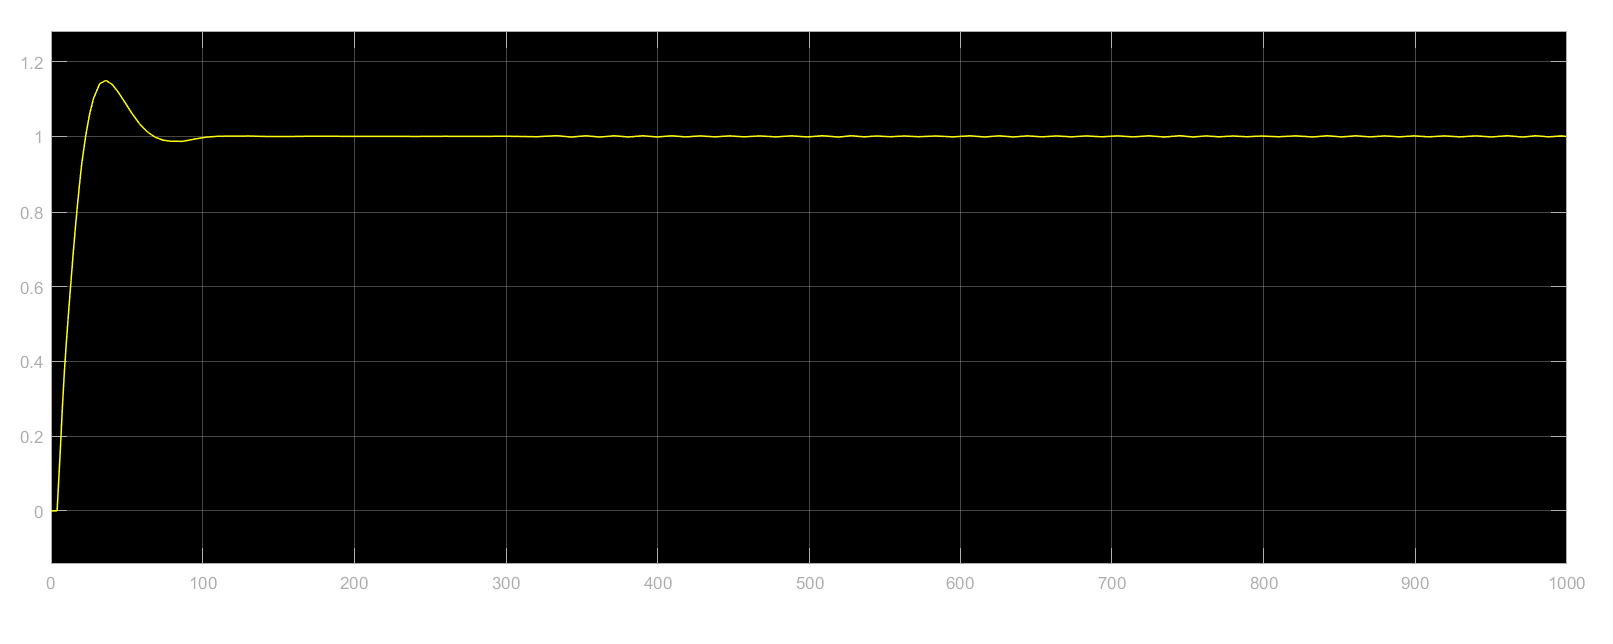
\includegraphics[scale=.50]{ap0239}
\caption{Az $A_P=0.2390$ rendszer ugrásválasza}
\end{figure}
A rendszer stabil így az $AP_P$ értékét $A_P=0.2460$-re növelem.
\begin{figure}[H]
\centering
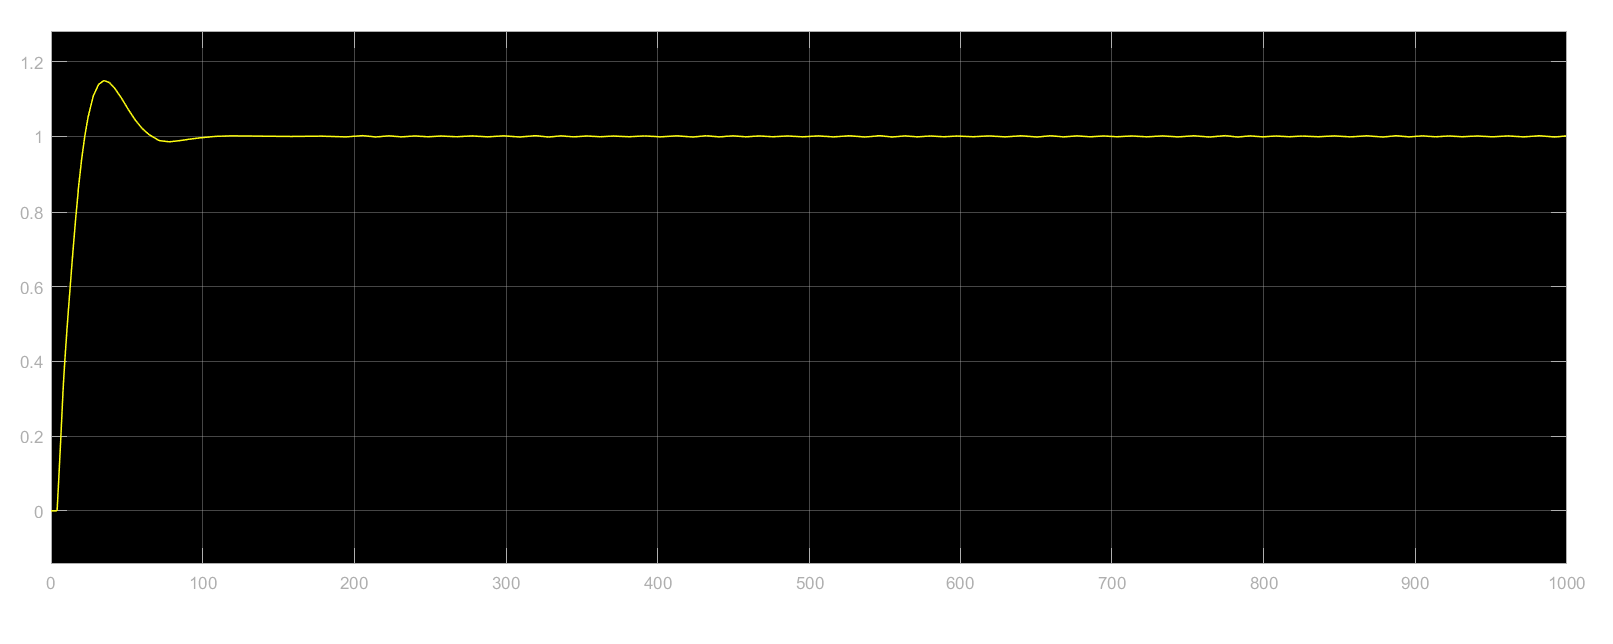
\includegraphics[scale=.50]{ap0246}
\caption{Az $A_P=0.2460$ rendszer ugrásválasza}
\end{figure}
A rendszer stabil így az $A_P$ értékét $A_P=0,2500$-re növelem.
\begin{figure}[H]
\centering
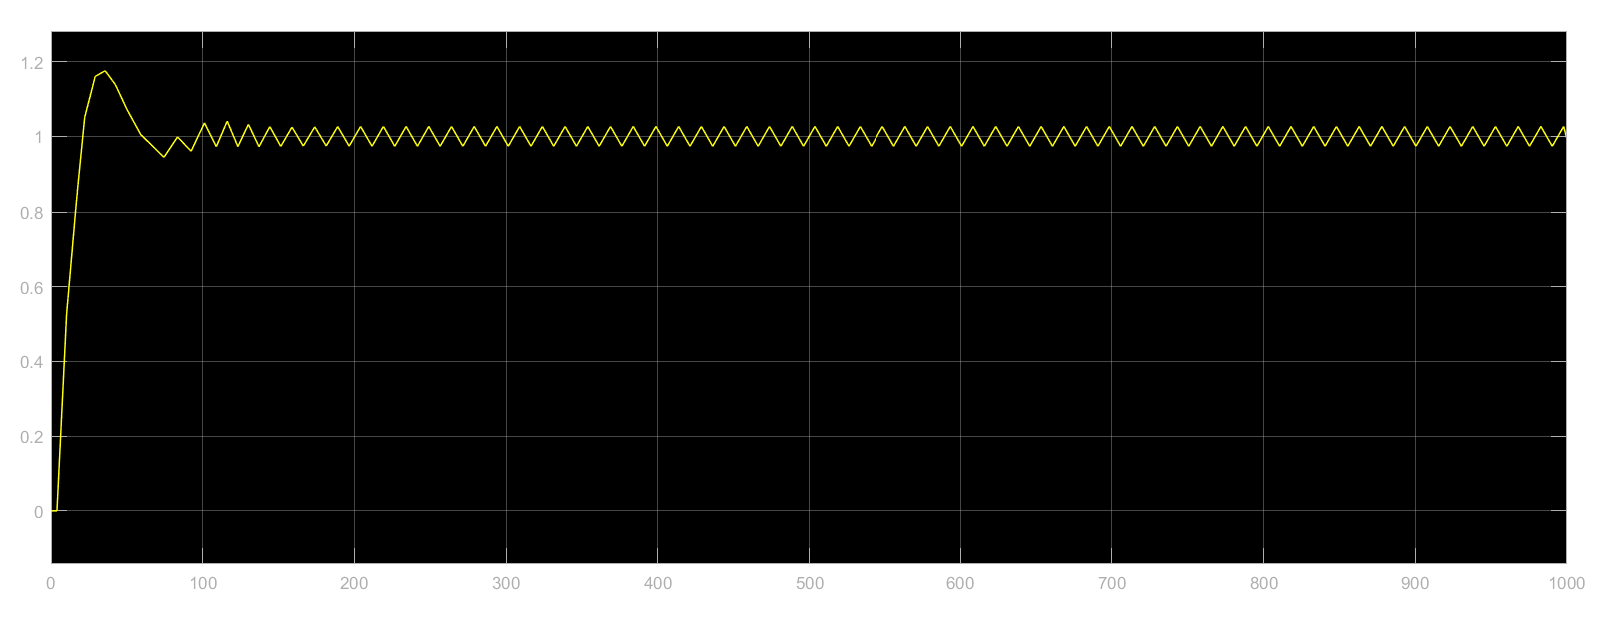
\includegraphics[scale=.50]{ap02500}
\caption{Az $A_P=0.2500$ rendszer ugrásválasza}
\end{figure}
A rendszer a stabilitás határán van, így az $A_P$ értékét $A_P=2482$-re csökkentem.
\begin{figure}[H]
\centering
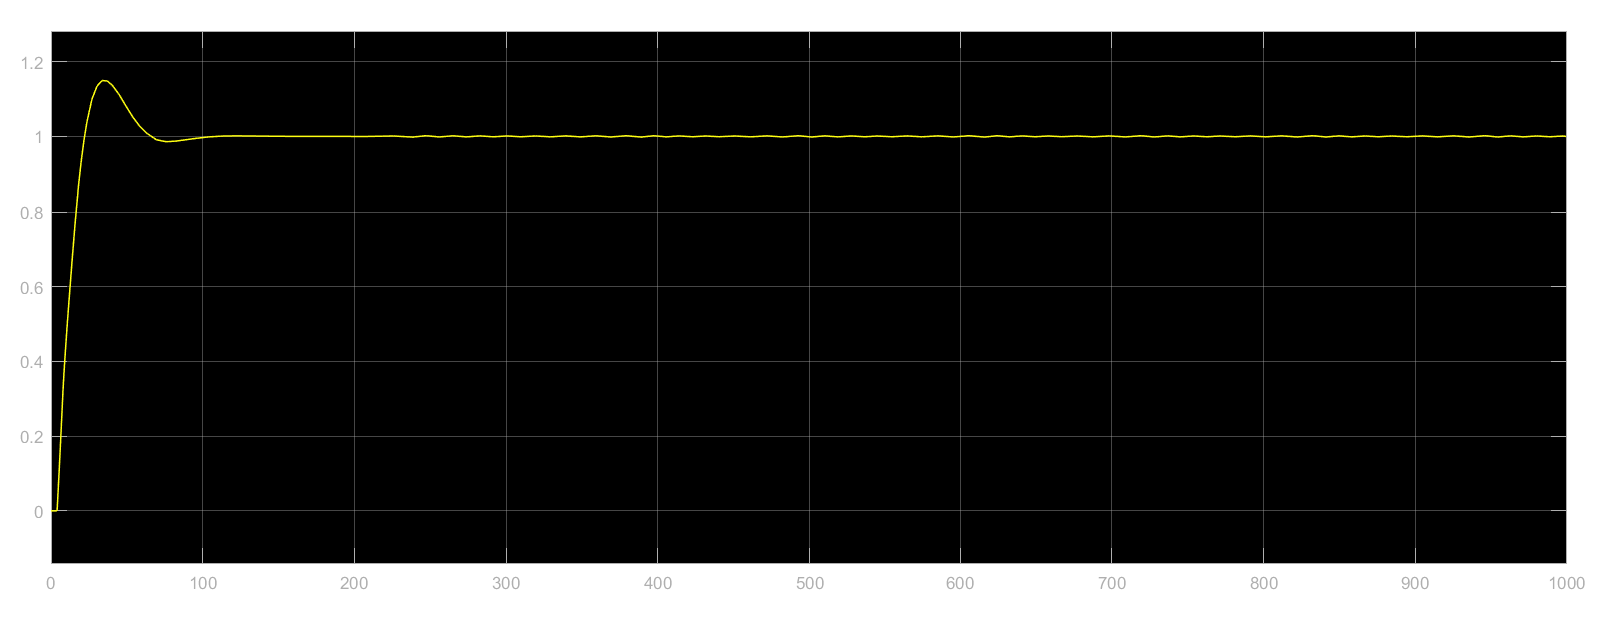
\includegraphics[scale=.50]{ap02482}
\caption{Az $A_P=0.2482$ rendszer ugrásválasza}
\end{figure}
A rendszer stabil, így 3 tizedesjegy pontosságra térve, az $A_P$ erősítést $A_P=.0249$ értékre növeltem, mivel látható, hogy $A_P=0.250$ estén már a stabilitás határán van a rendszer.
\begin{figure}[H]
\centering
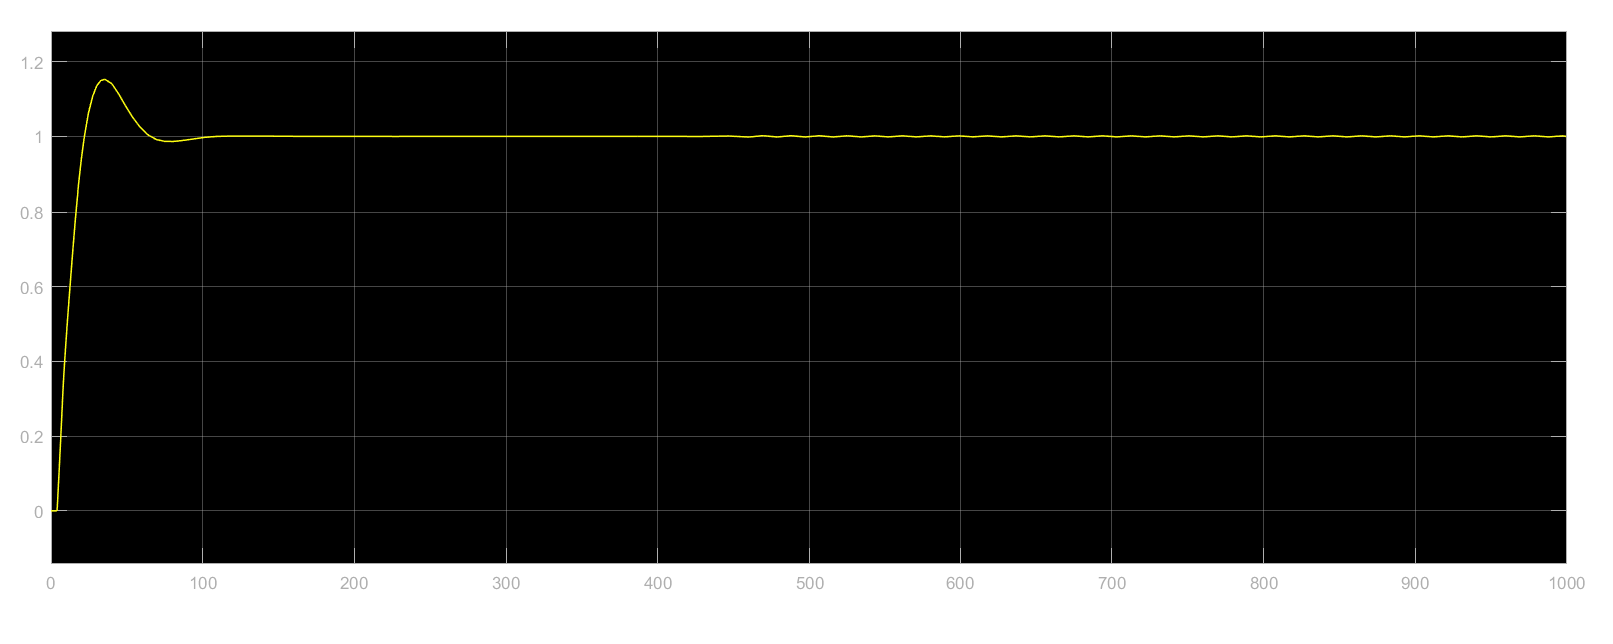
\includegraphics[scale=.50]{ap0249}
\caption{Az $A_P=0.249$ rendszer ugrásválasza}
\end{figure}
A rendszer stabil, van egy túllövése, majd egy alul lövést követve beáll a rendszer állandósult állapotba. A mérések alapján kijelenthető, hogy $A_P=0.249$ erősítésig lehet a rendszert erősíteni.

\subsection{PI szabályozó tervezés Ziegler-Nichols stabilitás határának elérésén alapuló szabályozás módszerével}
Adott átviteli függvény:
\[W_p(s)=\frac{1}{(1+12.4s)(1+5s)(1+1.3s)}e^{-T_us}\]
ahol $T_us=3$
A rendszer tartalmaz késleltetést $T_us=3$, amit Simulink alatt összeállítottam, ahol az stabilitás határának eléréséig egy $K_u$ erősítési a tényezővel állítottam.
\begin{figure}[H]
\centering
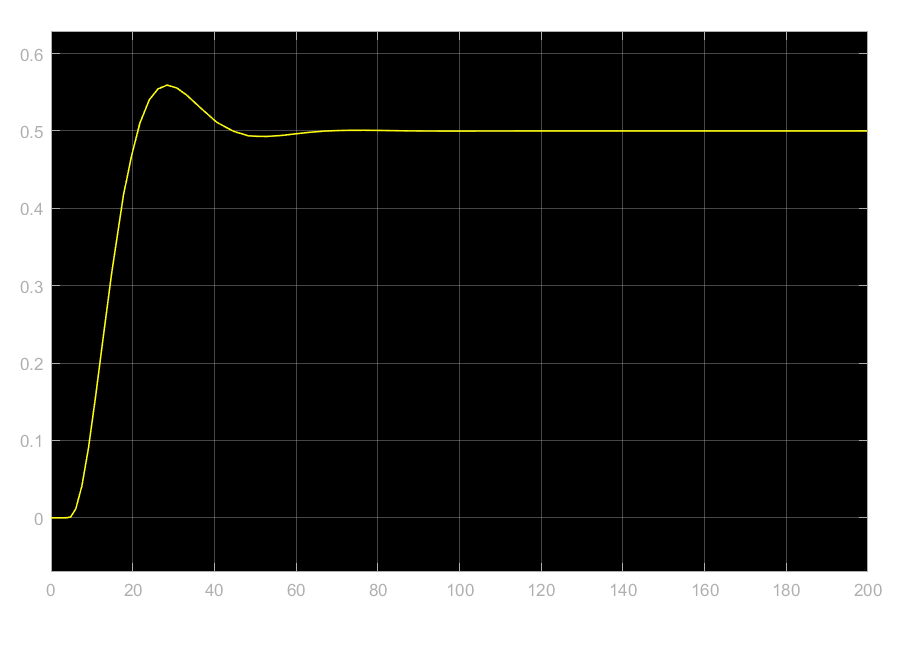
\includegraphics[scale=.70]{ZNSKU1}
\caption{Az $K_u=1$ erősítési tényezővel, a rendszer ugrásválasza}
\end{figure}
$K_u=1$ esetén, a rendszer stabilnak tűnik. Van túllövés, illetve azt követi egy alul lövés, majd beáll állandósult állapotba. Ez alapján véletlenszerűen, empirikus módon az erősítést növeltem $K_u=5$-re.
\begin{figure}[H]
\centering
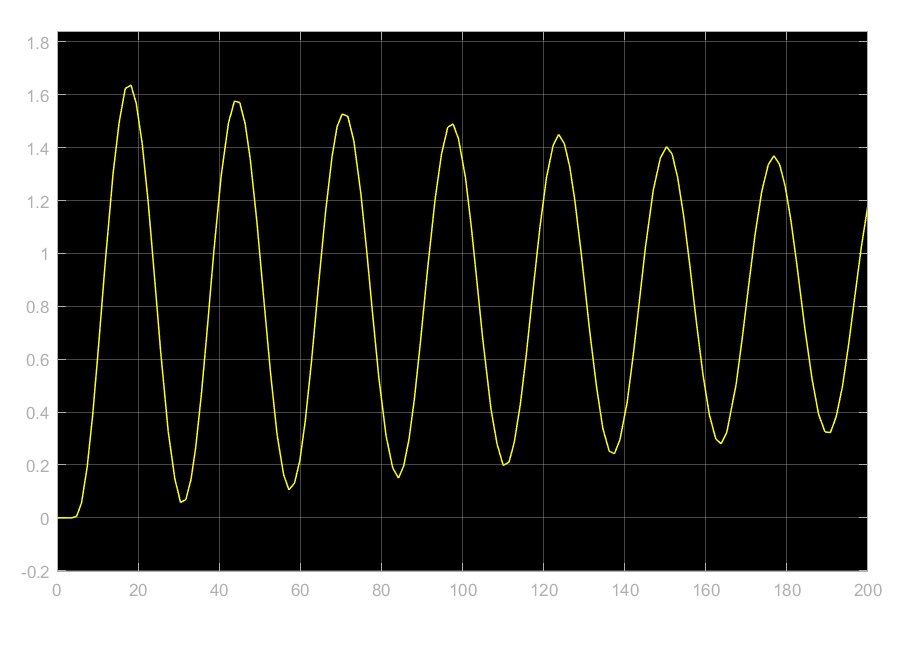
\includegraphics[scale=.70]{ZNSKU5}
\caption{Az $K_u=5$ erősítési tényezővel, a rendszer ugrásválasza}
\end{figure}
A rendszer itt már beleng, a stabilitás határán van. Viszont lehet látni, hogy kezd csillapodni. Az erősítést $K_u=5.5$-re tovább emelem.
\begin{figure}[H]
\centering
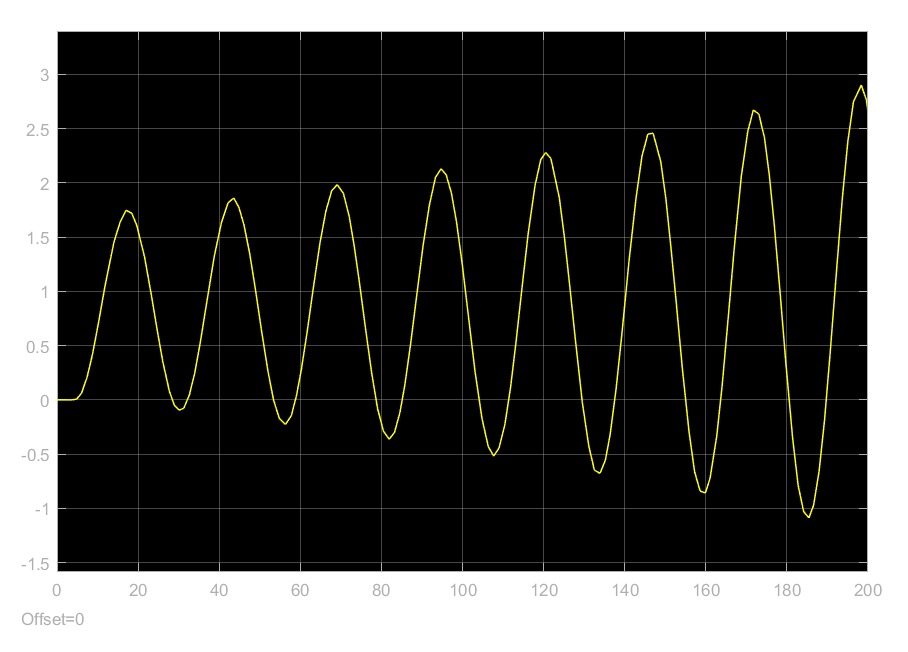
\includegraphics[scale=.70]{ZNSKU55}
\caption{Az $K_u=5.5$ erősítési tényezővel, a rendszer ugrásválasza}
\end{figure}
A rendszer instabil, így az optimális erősítés $5<K_u<5.5$ helyen található. Empirikus próbálkozások után $K_u=5.167$ esetén van a stabilitás határán.
\begin{figure}[H]
\centering
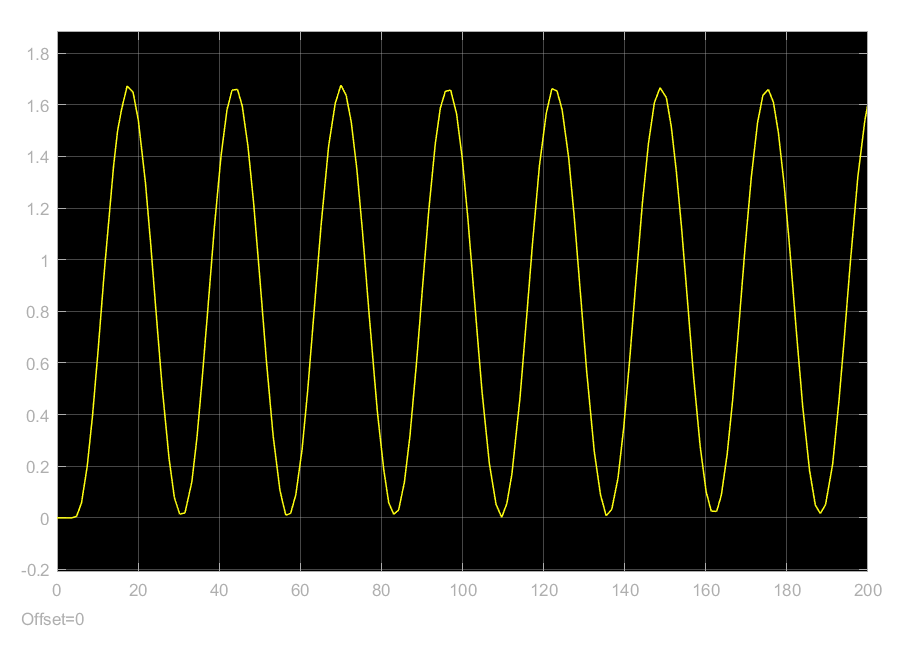
\includegraphics[scale=.70]{ZNSKU5167}
\caption{Az $K_u=5.167$ erősítési tényezővel, a rendszer ugrásválasza}
\end{figure}
Az ugrásválasz alapján leolvasom a két közeli kilengési ponton a periódus időt, ami $P_u=26.174$.
\begin{figure}[H]
\centering
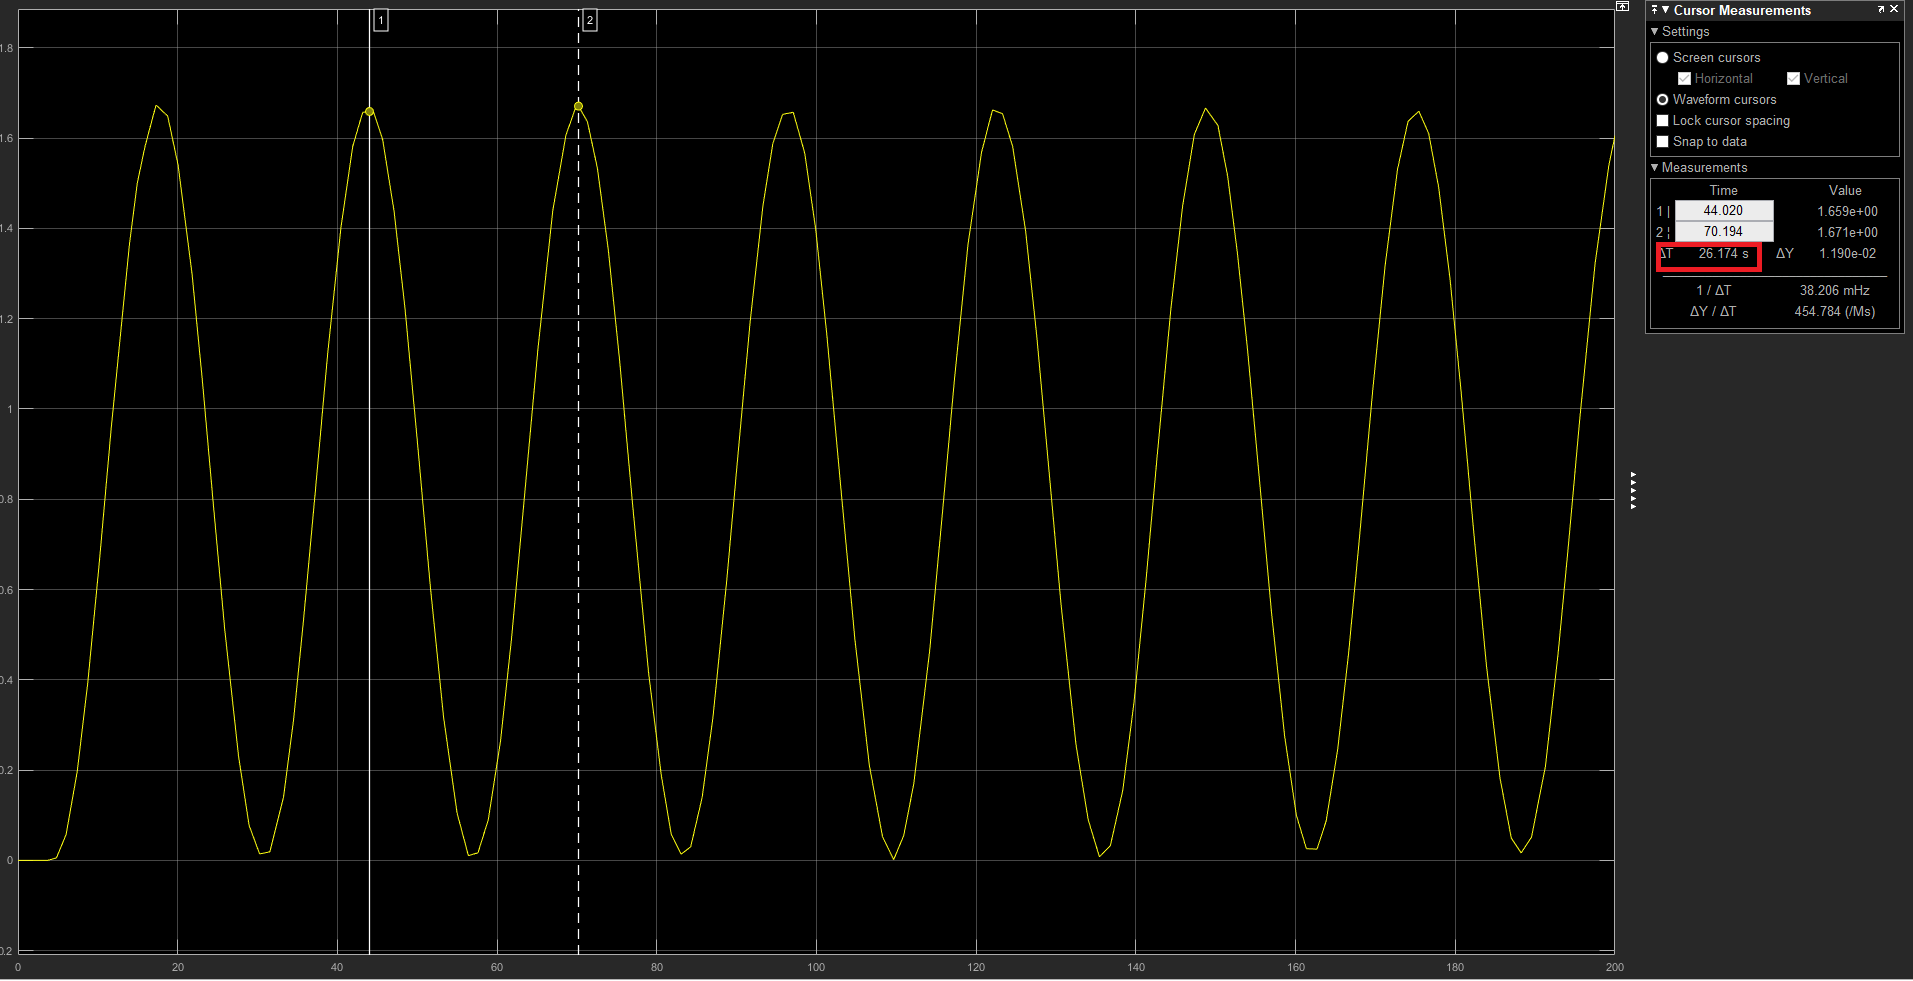
\includegraphics[scale=.30]{ZNSKPERIOD}
\caption{Az ugrásválaszból leolvasott $P_u=26.174$ periódus idő}
\end{figure}
PI szabályozó esetén így ki tudjuk számolni a 
\[A_p=0.45*K_u=0.45*5.167=2.325 \]
\[T_I=0.85*P_u=0.85*26.174=22.247 \]
A PI szabályozó átviteli függvénye:
\[WPI=A_p*(1+\frac{1}{sT_I})=2.325*(1+\frac{1}{22.247s})=\frac{51.73s+2.325}{22.25s}\]
A PI szabályozó átviteli függvényét elhelyeztem Simulink kapcsolásba az erősítés helyére.
Az ugrásválasz:
\begin{figure}[H]
\centering
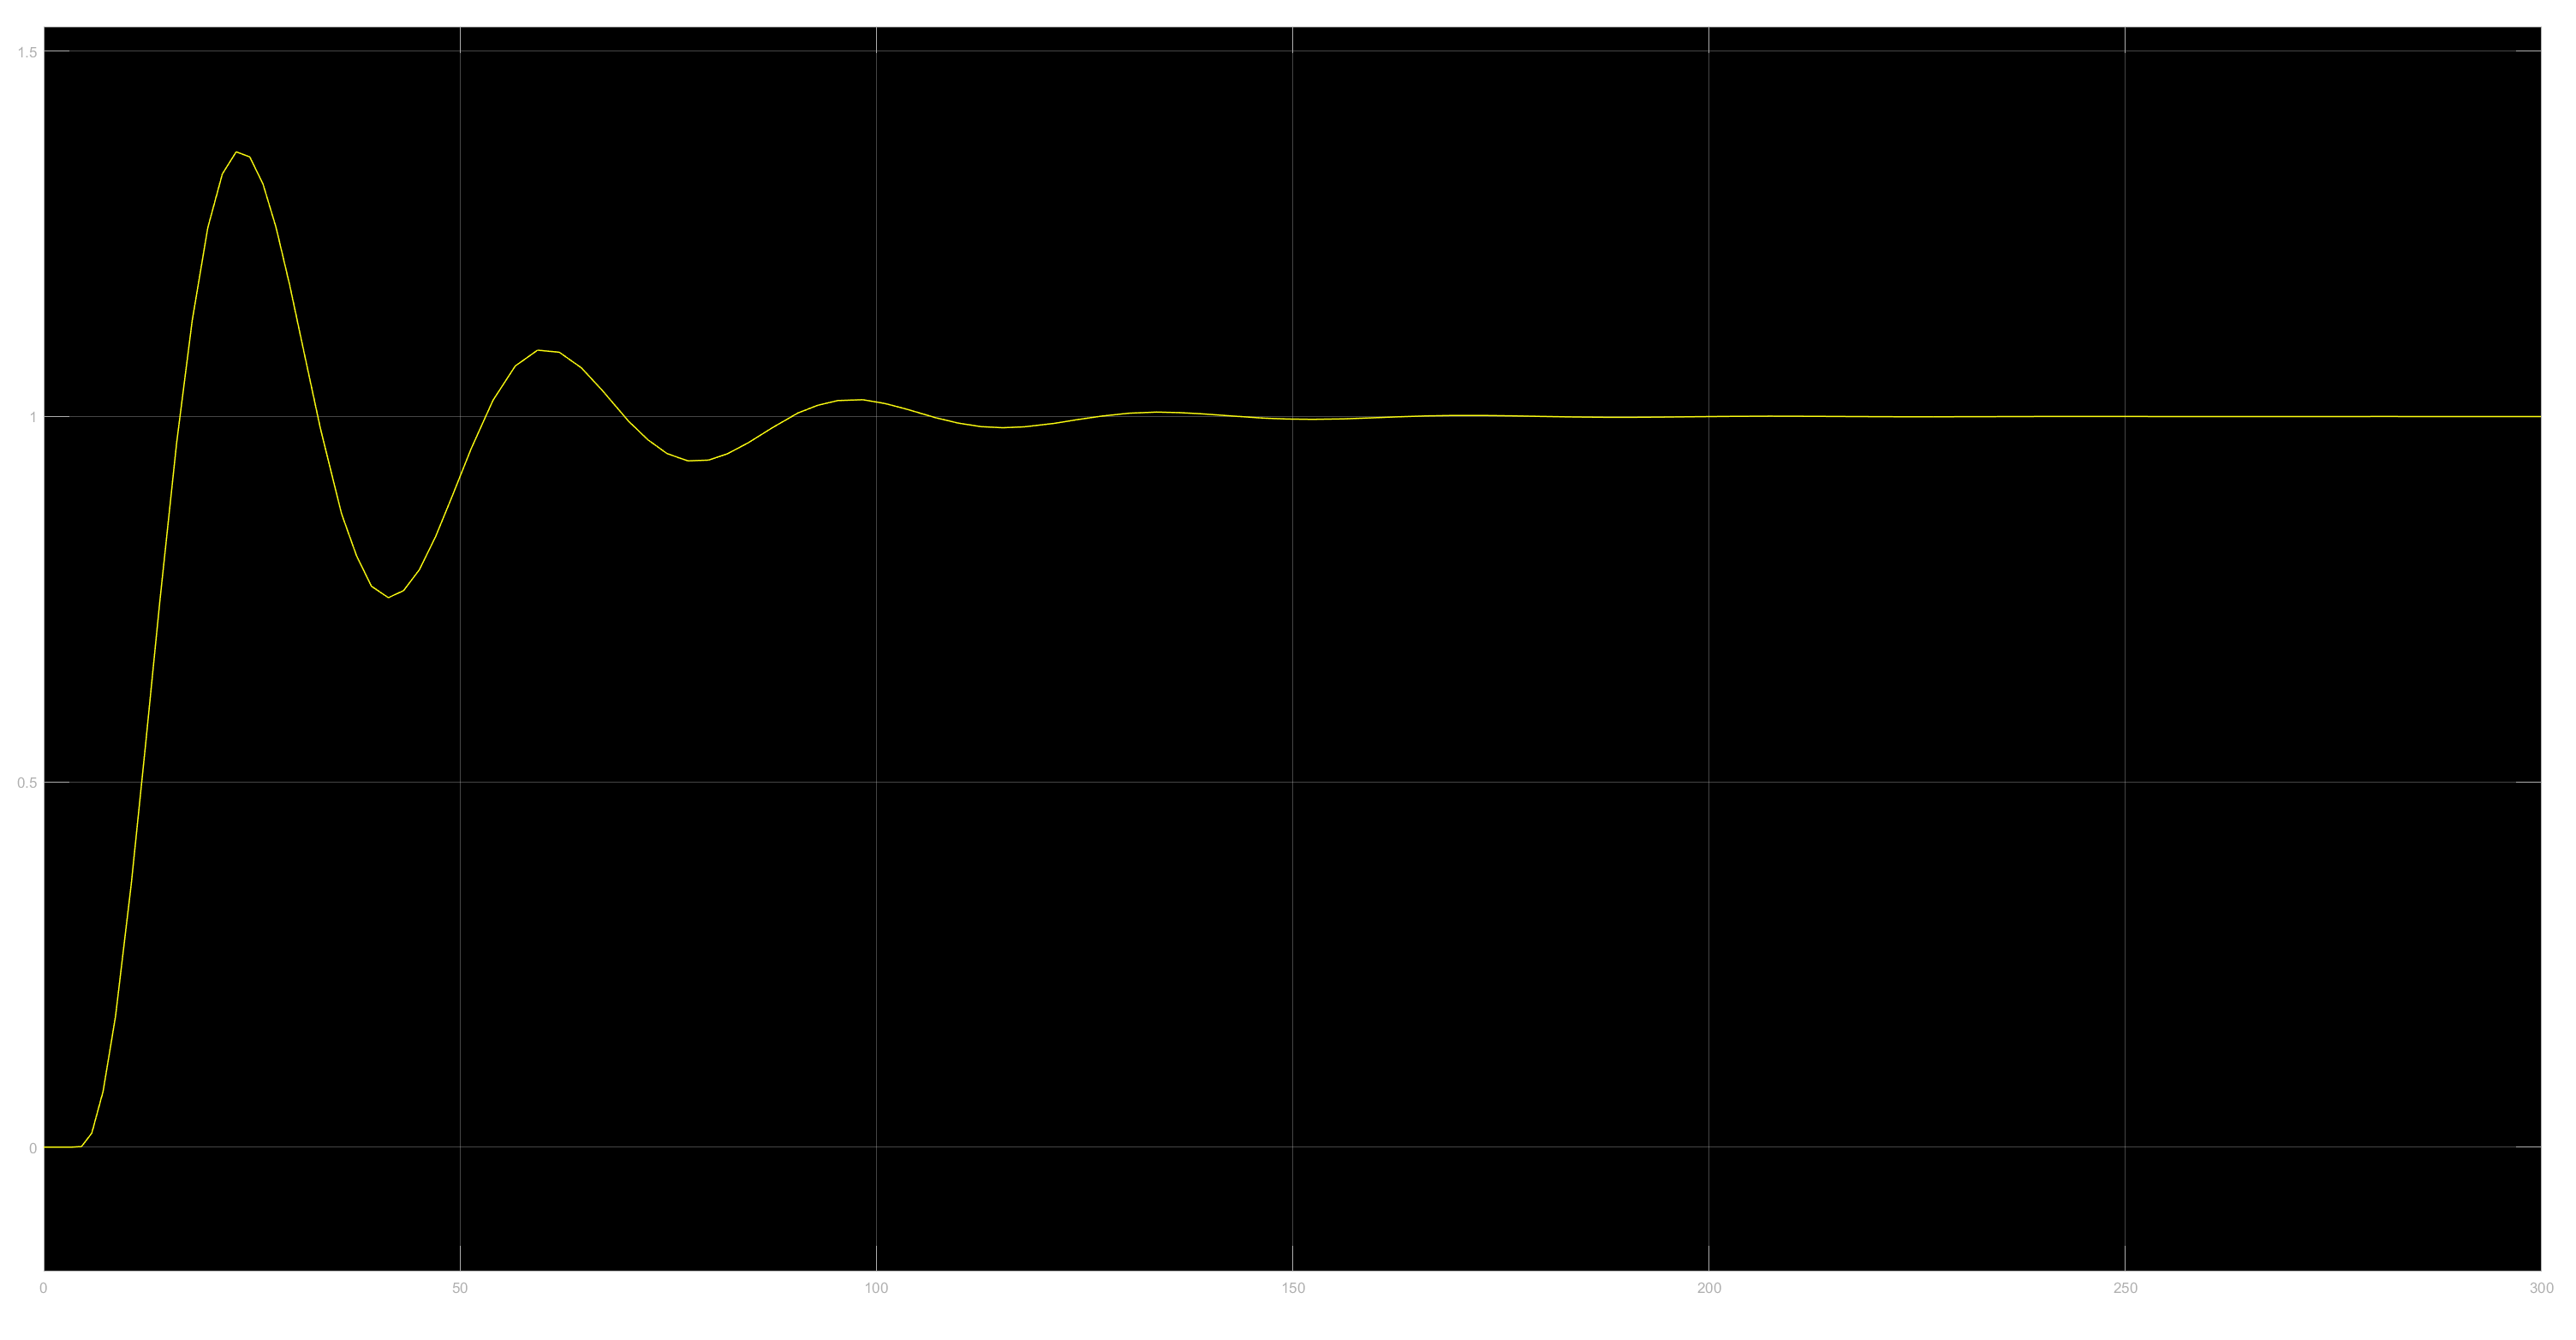
\includegraphics[scale=.30]{ZNSKUPI}
\caption{A tervezett PI szabályozóval, a rendszer ugrásválasza}
\end{figure}
A rendszer stabil, 1-re áll be a szabályozó, előtte van túllövése 1,3 majd 1,1 környékén. Végül 150s-nél beáll a rendszer.
\end{document}